
\section{Constructing Virtual Quality Levels by Skipping Frame Data}
\label{sec:virtual_quality_levels}


    In this section, we investigate whether intermediate quality levels—beyond the
    explicitly defined scalability layers—can be created by partially omitting
    enhancement-layer data.

    As described in Section~\ref{sec:svc_bitstream_structure}, the SVC bitstream is
    composed of access units, each containing slices corresponding to different
    enhancement layers. Each slice includes a slice header and a slice data section,
    which holds a list of macroblocks. These macroblocks are the smallest coding
    units in the video and contain motion, prediction, and residual data used by the
    decoder to reconstruct the frame.

    The structure of slice data for SVC bitstream is shown in
    Figure~\ref{fig:slice-data-syntax}.  Within the
    \texttt{slice\_data\_in\_scalable\_extension()} syntax, the
    \texttt{mb\_skip\_flag} is used to indicate that a macroblock is skipped.

    When a macroblock is skippped, motion vectors or residuals are not
    explicitly coded. Thus,
    \texttt{macroblock\_layer\_in\_scalable\_extension()} which contains the
    macroblock information is empty.

    This skipping mechanism applies only to P and B macroblocks, which use inter
    prediction. I macroblocks, which rely solely on intra prediction, cannot be
    skipped and must always be fully encoded.

    \begin{figure}
        \centering
        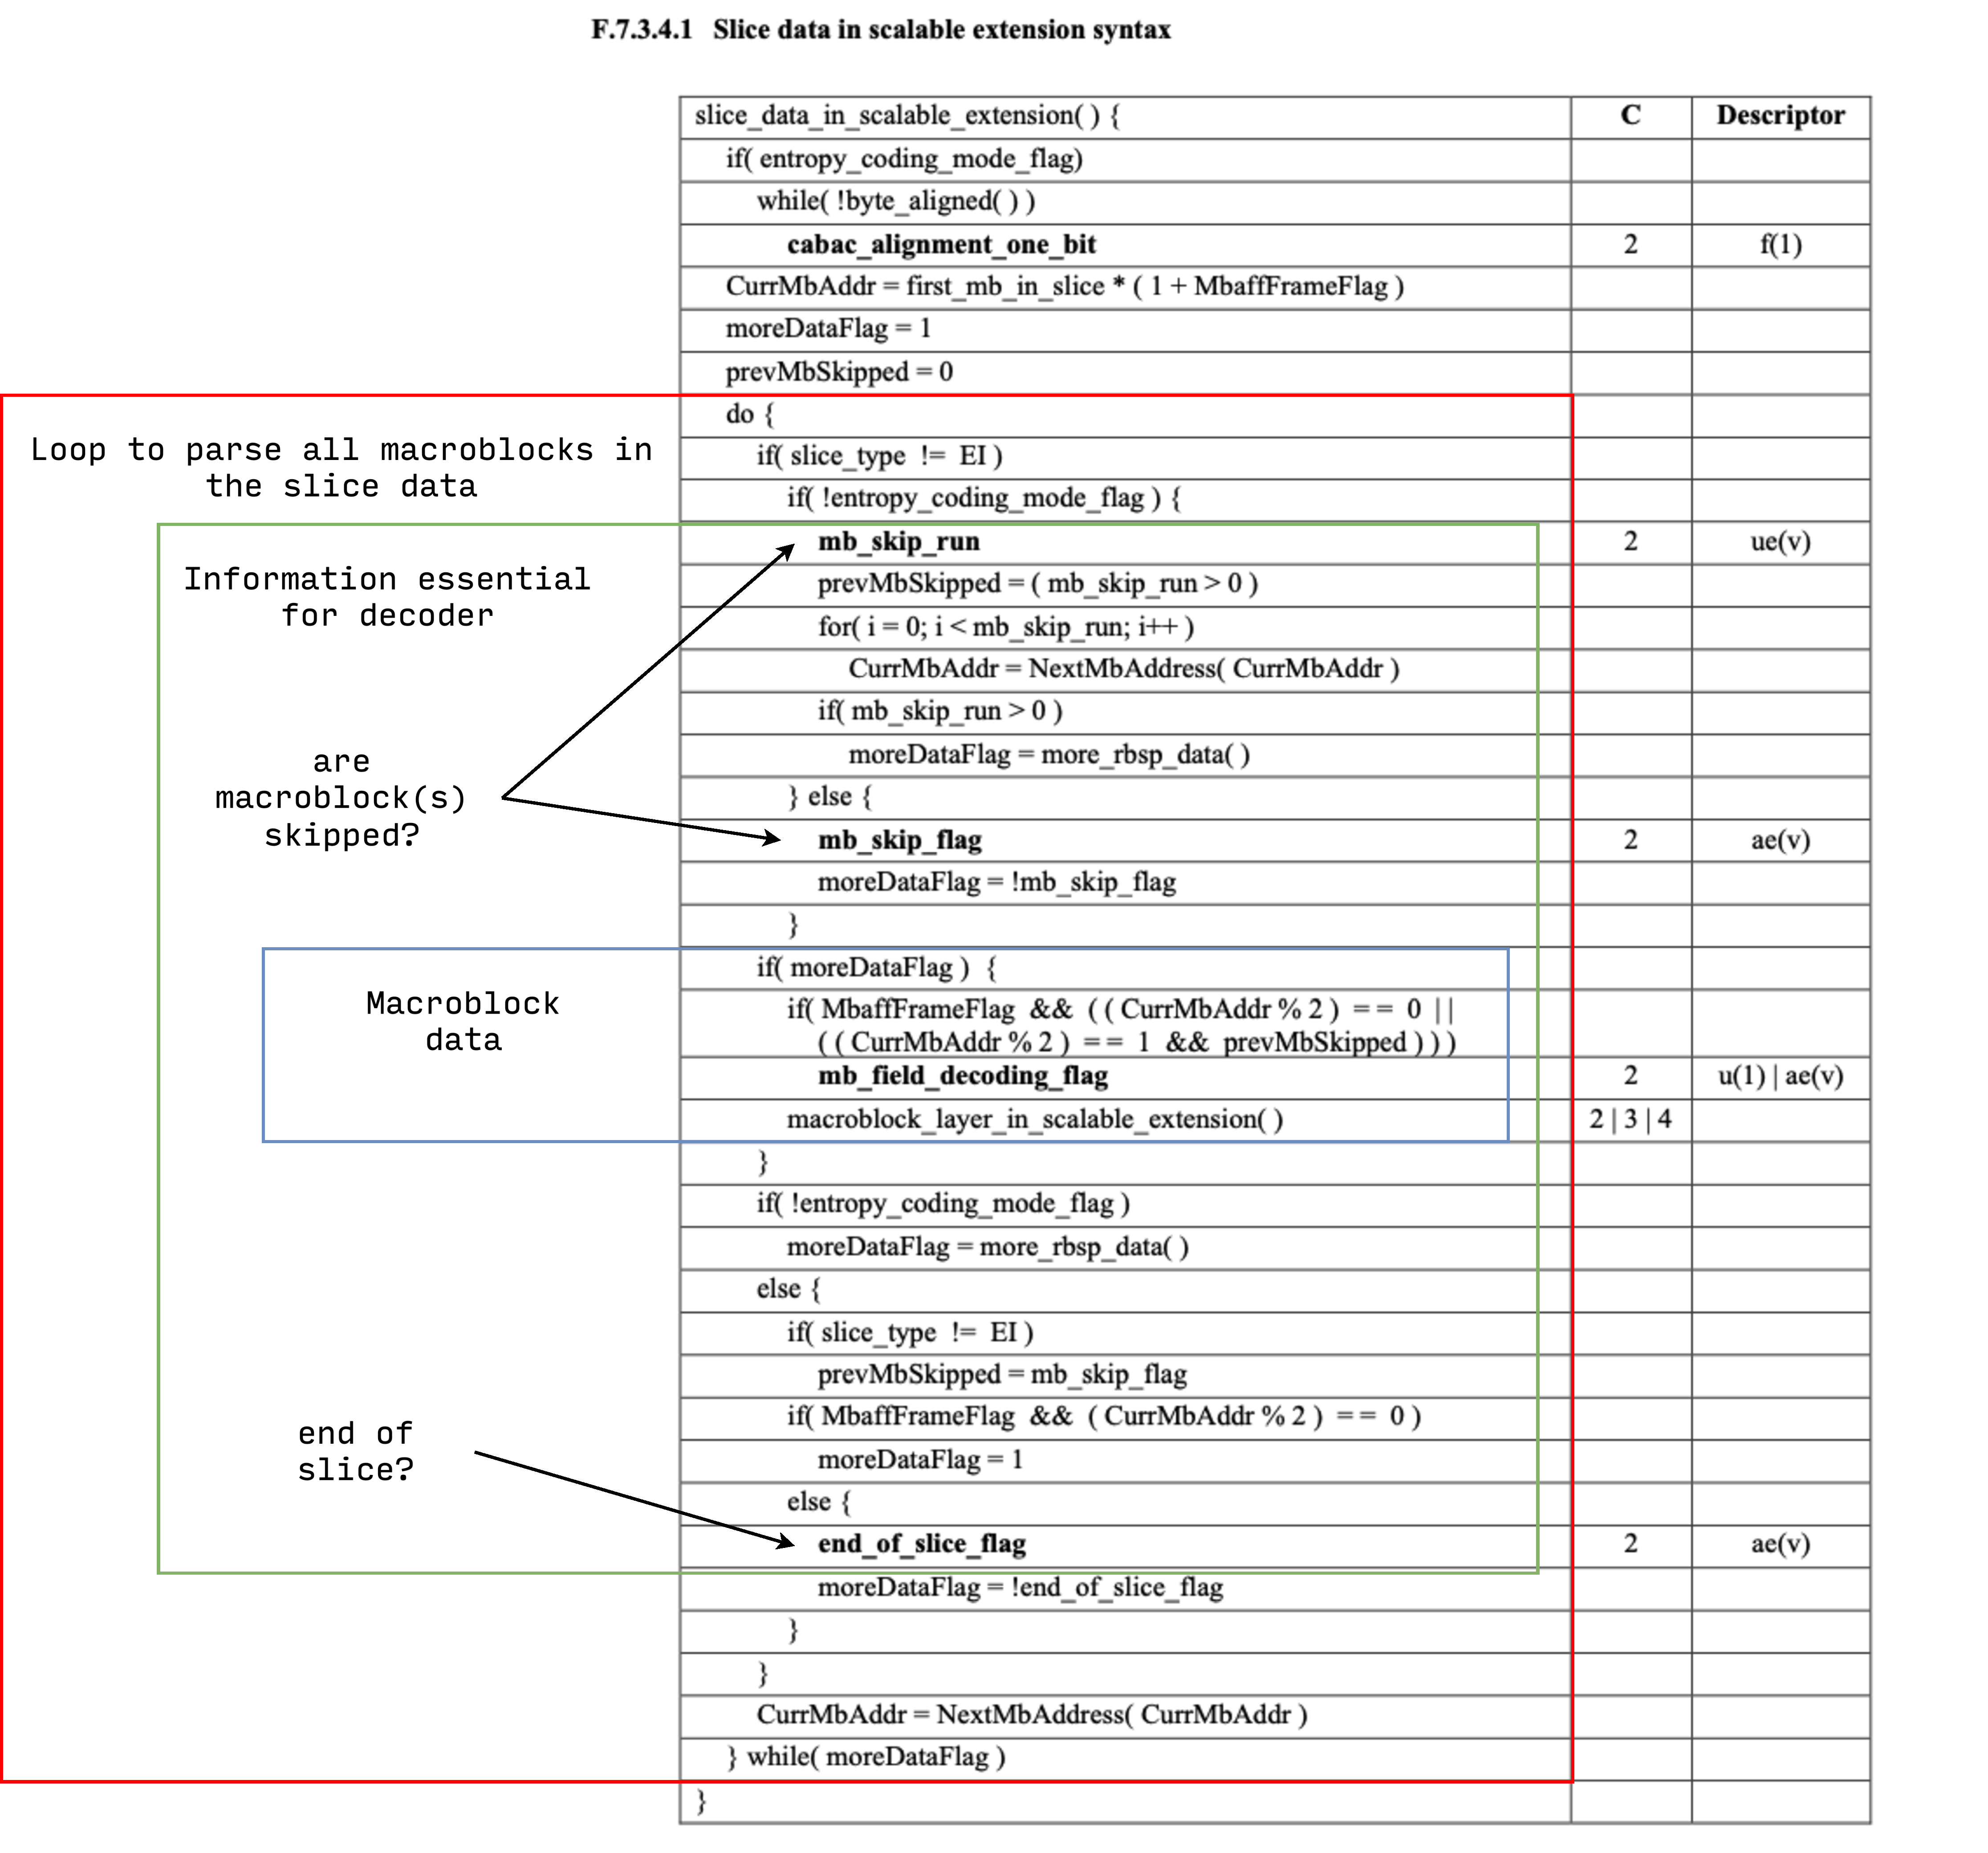
\includegraphics[width=\linewidth]{slice-data-syntax.pdf}
        \caption{Slice Data Syntax in H.264/SVC}
        \label{fig:slice-data-syntax}
    \end{figure}

    The macroblock skip mode in H.264 is primarily intended to improve compression
    efficiency by exploiting spatial and temporal similarities between frames. When
    the content of a macroblock closely matches a corresponding region in a
    reference frame, the encoder may mark it as skipped. Instead of encoding new
    data, the decoder reconstructs the macroblock using prediction. This often
    requires only a single bit to signal skipping via the \texttt{mb\_skip\_flag},
    reducing the bitrate with minimal impact on visual quality.

    In our approach, we take advantage of this mechanism to selectively skip
    macroblocks in the enhancement layers. For each macroblock marked for omission,
    we set the \texttt{mb\_skip\_flag} and remove the associated
    \texttt{macroblock\_layer\_in\_scalable\_extension()} data from the bitstream.
    This enables fine-grained control over which parts of the enhancement data are
    retained, allowing us to simulate continuous quality variations rather than
    relying solely on predefined SVC layer switching.

    These selectively modified bitstreams result in what we refer to as
    \textit{virtual quality levels}—intermediate representations that provide
    smoother adaptability and more flexible quality trade-offs. In the following
    sections, we evaluate the visual impact of these virtual quality levels using
    objective metrics such as SSIM, PSNR, and VMAF, and assess their potential to
    improve streaming performance under network constraints.


\section{Motion and Residual and Upsampling}
